% JORS Software Metapaper: quantum-group
%
% Structure follows the JORS Software Metapaper template headings:
% (1) Overview [Title, Paper Authors, Paper Author Roles and Affiliations,
% Abstract, Keywords, Introduction, Implementation and architecture, Quality
% control], (2) Availability [Operating system, Programming language,
% Additional system requirements, Dependencies, List of contributors,
% Software location (Archive, Code repository), Language], (3) Reuse
% potential; followed by the statements listed in the journal's suggested
% structure (Data Accessibility, Acknowledgements, Funding Information,
% Competing Interests, Authors' Contributions) and a generative-AI statement
% required by the Ubiquity Press policy. See jors/PREFLIGHT.md for how the
% current rules were checked.
%
% Author- and event-dependent facts live in submission-facts.tex.
% Build (from jors/):  make  (or latexmk -pdf paper.tex)
\documentclass[11pt,a4paper]{article}

\usepackage[T1]{fontenc}
\usepackage[utf8]{inputenc}
\usepackage{lmodern}
\usepackage[british]{babel}
\usepackage{csquotes}
\usepackage[margin=25mm]{geometry}
\usepackage{amsmath,amssymb}
\usepackage{graphicx}
\usepackage{booktabs}
\usepackage{tabularx}
\usepackage{array}
\usepackage{xcolor}
\usepackage{listings}
\usepackage{caption}
\usepackage{enumitem}
\usepackage{microtype}
\usepackage[backend=biber,style=vancouver,sorting=none,maxnames=6,minnames=6]{biblatex}
\usepackage[hidelinks]{hyperref}
\usepackage{xurl}

\addbibresource{references.bib}
% Vancouver form "Place: Publisher; year. p. x-y." for proceedings chapters.
\DeclareFieldFormat[inproceedings]{pages}{\unskip.\space p.~\mkcomprange{#1}}

\setlength{\parskip}{0.45em}
\setlength{\parindent}{0pt}
\setlist{itemsep=0.15em, topsep=0.25em}
\captionsetup{font=small, labelfont=bf}

% Values that can only be supplied by the author or an external event are
% defined in submission-facts.tex; unresolved ones print as red markers.
\newcommand{\pending}[1]{\textcolor{red!70!black}{\textbf{[PENDING: #1]}}}
% Facts that only the author or an external event can supply.
%
% Every value below that is still \pending{...} is printed in red in the PDF,
% so an incomplete manuscript cannot be mistaken for a final one. Replace each
% \pending{...} with the confirmed text; `make -C jors check` (see
% jors/Makefile) fails while any \pending remains in the rendered PDF.
% Do not fill a field with a guess.

% --- Author declarations -------------------------------------------------
\newcommand{\AuthorAffiliation}{\pending{current affiliation}}
\newcommand{\FundingText}{\pending{funding statement}}
\newcommand{\CompetingText}{\pending{competing-interests statement}}
% AI use during the April--June 2026 thesis/core-development period.
\newcommand{\ThesisPeriodAI}{\pending{AI use during April--June 2026: none, or tool/model/scope}}
% Model names exactly as confirmed by the author.
\newcommand{\ClaudeModel}{\pending{Claude model name(s)/version(s)}}
\newcommand{\CodexModel}{\pending{Codex model name/version}}
% Confirmation that all AI-assisted output was human reviewed and validated.
\newcommand{\AIReviewStatement}{\pending{author's confirmation of human review and validation of all AI-assisted output}}

% --- Software snapshot and distribution ----------------------------------
% Exact commit described by the paper (the JORS submission software snapshot).
\newcommand{\SnapshotSHA}{\pending{snapshot commit SHA}}
\newcommand{\SnapshotDate}{\pending{snapshot commit date}}
% Zenodo software deposition of `git archive` of the snapshot commit.
\newcommand{\ArchiveDOI}{\pending{Zenodo DOI of the 1.1.0 snapshot}}
\newcommand{\ArchiveDate}{\pending{Zenodo publication date}}
% PyPI: public once `python -m pip install quantum-group==1.1.0` works.
\newcommand{\PyPIIdentifier}{\pending{PyPI publication of quantum-group 1.1.0}}


\newcommand{\pkg}{\texttt{quantum-group}}
\newcommand{\code}[1]{\texttt{#1}}
\newcommand{\Uq}{U_q(\mathfrak{sl}_2)}
\newcommand{\GL}{GL_q(2|1)}

\lstset{basicstyle=\ttfamily\small, columns=fullflexible, keepspaces=true,
  frame=single, framerule=0.4pt, rulecolor=\color{black!40},
  xleftmargin=4pt, xrightmargin=4pt, aboveskip=0.6em, belowskip=0.4em,
  commentstyle=\color{black!60}, showstringspaces=false, upquote=true}

\begin{document}

\section*{(1) Overview}

\subsection*{Title}

{\Large\bfseries \pkg: Exact SymPy Verification of Explicit $\Uq$ and $\GL$ Matrix Identities\par}

\subsection*{Paper Authors}

1. Terekli, Taha Berk \\ ORCID: \href{https://orcid.org/0009-0004-8266-1116}{0009-0004-8266-1116}\\ Corresponding author: \href{mailto:terekli@tahaberk.com}{terekli@tahaberk.com}

\subsection*{Paper Author Roles and Affiliations}

1. \AuthorAffiliation. Sole developer and maintainer of the software; author of this paper.

\subsection*{Abstract}

\pkg{} is an open-source Python package for checking explicit matrix identities from the theory of quantum groups. Checking a Yang--Baxter equation, an R-matrix's compatibility with a coproduct, or a defining relation is error-prone by hand, since the answer depends on basis order, tensor placement, the coproduct and, for superalgebras, sign rules. The package builds the matrices exactly with SymPy and returns each identity as an exact residual matrix whose entries must simplify to zero. It covers finite-dimensional $\Uq$ modules, their tensor products and fundamental R-matrix, and the graded R-matrix of the quantum supergroup $\GL$ of Çelik and Çelik. Applied to the author's own undergraduate thesis, it caught a real convention error that the usual Yang--Baxter test had not revealed. Researchers can check published matrices in their own conventions and keep the checks as regression tests. It is MIT-licensed, on GitHub, PyPI and Zenodo.

\subsection*{Keywords}

quantum groups; symbolic computation; SymPy; R-matrix; Yang--Baxter equation; Lie superalgebras; computer algebra; reproducible research

\subsection*{Introduction}

Quantum groups are one-parameter deformations of classical symmetry algebras. Their representations yield solutions of the quantum Yang--Baxter equation (QYBE), which is why they appear in exactly solvable models of statistical mechanics, in knot invariants and in representation theory \cite{drinfeld1987,jimbo1985,jimbo1986,kassel1995}. Much of the working knowledge in this area is recorded as explicit matrices whose entries are rational functions of the deformation parameter $q$: an R-matrix on $V\otimes V$, the generators of a module, a change of basis to irreducible summands. Before such a matrix can be reused it has to be checked, and checking it means multiplying $9\times9$, $27\times27$ or $81\times81$ matrices whose meaning depends on conventions that texts state in different ways, or not at all.

The characteristic mistakes are not arithmetic ones. A matrix is transcribed in a different basis order from the one its source used. $R_{13}$ is formed by conjugating with the wrong permutation. An R-matrix is paired with the opposite of the coproduct it actually intertwines; this still satisfies the QYBE, so the most common test does not detect it. In a $\mathbb{Z}_2$-graded setting an ordinary flip is used where the Koszul sign rule requires a super-permutation. And a check that is run at a floating-point value of $q$ can hide cancellations or produce spurious nonzero entries. Each of these errors produces output that looks plausible.

\pkg{} addresses this with a deliberately narrow design. Every object is an ordinary exact \code{sympy.Matrix} \cite{meurer2017sympy}; conventions (basis order, coproduct, parities) are fixed in documented functions; and every identity is exposed as a \emph{residual}, the exact matrix $\mathrm{LHS}-\mathrm{RHS}$, which is then tested entry by entry. For $\Uq$ the package constructs the irreducible modules $V_n$, checks the defining relations and generator-level Hopf identities, builds tensor products through the coproduct, computes Clebsch--Gordan highest-weight vectors, and verifies the fundamental R-matrix: QYBE, braid and Hecke relations and coproduct intertwining. For the quantum supergroup $\GL$ introduced by Çelik and Çelik \cite{celik2021}, whose third basis vector is odd, it constructs the published $9\times9$ R-matrix and verifies the graded Yang--Baxter equation on three factors and on every triple of factors in $V^{\otimes4}$.

The software was developed for and used in the author's undergraduate thesis \cite{terekli2026thesis}, where it produced the thesis's tables, matrix figures and Yang--Baxter verifications. After the thesis was submitted in June 2026, the software was used to audit it: an explicit intertwining residual showed that the thesis's R-matrix intertwines the opposite of the coproduct used in the text, an error that passing QYBE, braid and Hecke checks had not revealed. The correction is recorded in the repository (\code{thesis/ERRATA.md}, \code{AUDIT.md}), and the check is now part of the API and the test suite. No new mathematical results are claimed here; the contribution is the software and its verification method.

The intended users are researchers who need to confirm a matrix identity from the literature in their own conventions, mathematical physicists working with R-matrices, representation theorists and computer-algebra users who want an inspectable reference calculation, and students reproducing standard quantum-group computations.

\emph{Related software.} GAP's QuaGroup package \cite{gap,quagroup,degraaf2001} and SageMath \cite{sagemath}, which provides a \code{QuantumGroup} interface to it, work with the quantized enveloping algebra $U_q(\mathfrak{g})$ of any semisimple Lie algebra $\mathfrak{g}$: they construct PBW-type and canonical bases, highest-weight modules and their R-matrices; SageMath also implements crystals for the quantum superalgebras $U_q(\mathfrak{gl}(m|n))$ \cite{bkk2000}. These systems are far broader, and for general $U_q(\mathfrak{g})$ work they are the appropriate tools. \pkg{} does not replace them. It is a small verification layer for concrete matrix calculations: it keeps the basis order and coproduct of a particular text, returns the matrices themselves, runs in an ordinary Python environment, and includes a graded $\GL$ example that lies outside QuaGroup's documented $U_q(\mathfrak{g})$ scope.

\emph{Scope and limitations.} A zero residual establishes an identity on the particular finite-dimensional representation used; it is not a proof in the abstract Hopf algebra, and the package is not a theorem prover. It does not implement general quantum groups. For $\GL$ it implements the R-matrix, the graded Yang--Baxter equation and tensor placements, not the RTT relations, the Hopf superalgebra structure or the Gauss decomposition of \cite{celik2021}. It verifies the Hecke relation but does not compute a Markov trace or the Jones polynomial. Its root-of-unity helpers substitute special values into the generic construction; they do not implement the small quantum group. The crystal graph $B(n)$ is a combinatorial model rather than a crystal-basis algorithm.

\subsection*{Implementation and architecture}

\pkg{} is a pure-Python package of fifteen modules (about 2{,}000 lines, including docstrings) with no compiled extensions. Figure~\ref{fig:workflow} shows the workflow that the modules implement; the design decisions behind each step are described below.

\begin{figure}[t]
  \centering
  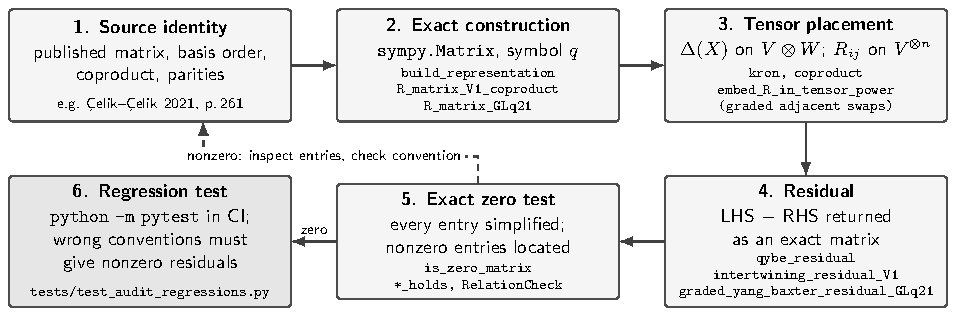
\includegraphics[width=\textwidth]{figures/figure1_workflow.pdf}
  \caption{Verification workflow in \pkg. A published identity and its conventions (1) are turned into exact SymPy matrices (2) and placed on tensor products through the coproduct or through graded adjacent swaps (3). The difference of the two sides is returned as an exact residual matrix (4) and tested entry by entry (5); a nonzero residual points to the entries, and hence the convention, that disagree. Zero residuals, and nonzero residuals for deliberately wrong conventions, are kept as regression tests (6). Function names are those of the public API.}
  \label{fig:workflow}
\end{figure}

\emph{Explicit matrices rather than an abstract algebra engine.} The package contains no noncommutative rewriting system; the symbols in \code{generators.py} only display the relations. Every check runs on concrete representation matrices. This keeps each object directly comparable, entry by entry, with a printed matrix, and makes every intermediate result an ordinary SymPy object that users can print, substitute into or pass to other SymPy code. The price is that a verification holds for the representations on which it is run, and that the cost grows with the dimension of the tensor product (see \emph{Scaling}). Identities that need a genuinely noncommutative graded algebra, such as the Gauss decomposition of $\GL$, are omitted rather than approximated with commuting symbols.

\emph{Layers.} The modules form three layers. A small foundation provides the default symbol $q$ (declared nonzero), $q$-integers, $q$-factorials and $q$-binomials (\code{utils}); the Kronecker product \code{kron}/\code{kron\_list} and the zero-residual test \code{is\_zero\_matrix} (\code{linalg}); and internal argument checks (\code{\_validation}). Construction modules build the matrices: $\Uq$ modules (\code{representations}), coproduct, counit and antipode (\code{hopf}), tensor products and Clebsch--Gordan vectors (\code{tensor}), $\Uq$ R-matrices (\code{r\_matrix}) and the $\GL$ R-matrix, super-permutation and embeddings (\code{supergroup\_gl21}). Verification functions sit next to the constructions they check and all use the same foundation. Auxiliary modules provide classical and root-of-unity specializations (\code{limits}), the crystal graph $B(n)$ as a NetworkX \cite{hagberg2008networkx} graph (\code{crystal}), Matplotlib \cite{hunter2007matplotlib} weight and crystal plots (\code{visualization}) and a convenience facade, \code{QuantumGroupSL2}. The main functions are re-exported from the package namespace and listed in \code{\_\_all\_\_}; a few helpers, such as \code{kron}, are imported from their modules (\code{quantum\_group.linalg}).

\emph{Residual-first verification.} Each check follows one pattern: build the left-hand side, build the right-hand side, return their difference, and decide whether every entry is zero. Functions named \code{*\_residual} (\code{qybe\_residual}, \code{braid\_relation\_residual}, \code{intertwining\_residual\_V1}, \code{graded\_yang\_baxter\_residual\_GLq21}, and others) return the exact difference matrix; the corresponding \code{*\_holds} functions apply \code{is\_zero\_matrix} to it; and \code{verify\_on\_representation} returns, for each defining relation, a \code{RelationCheck} record holding both the Boolean and the residual. Returning the residual rather than only a Boolean is what makes a failed check informative: the positions and values of the nonzero entries identify which basis vectors and which convention disagree. For example, placing the $\GL$ R-matrix with an ordinary flip instead of the super-permutation leaves exactly two nonzero entries of the $27\times27$ residual, both equal to $2q^2(q-1)^2(q+1)^2$ (Listing~\ref{lst:example}). The zero test simplifies each entry with \code{sympy.simplify}. A \code{True} result means that every entry was reduced to the exact value 0; a \code{False} result is not by itself a proof of inequality, because \code{simplify} is not a decision procedure. For the rational functions of $q$ produced by the package, a nonzero entry can be confirmed with \code{sympy.cancel}, which the regression tests do.

\emph{Exact parameters.} The default parameter is a nonzero SymPy symbol, and the identities are rational in $q$, holding wherever their denominators are defined. Integers and exact rationals passed as $q$ are converted to exact SymPy numbers, so \code{build\_representation(2, 2)} yields entries such as $5/2$ rather than $2.5$; only floating-point values supplied by the user are approximate. $q$-integers and $q$-binomials are evaluated as Laurent polynomials, not as quotients, so that specializations with removable singularities, such as $q=-1$ or roots of unity, give the correct values instead of $0/0$.

\emph{Representations and tensor products.} \code{build\_representation(n)} returns the $(n+1)$-dimensional module $V_n$ as a \code{Representation} record with explicit matrices $E$, $F$, $K$ and $K^{-1}$ in the basis $v_0,\dots,v_n$, where $K$ is diagonal, $F$ is a lower shift and $E$ carries the products of $q$-integers. The coproduct is fixed as
\[
\Delta(E)=E\otimes 1+K\otimes E,\qquad \Delta(F)=F\otimes K^{-1}+1\otimes F,\qquad \Delta(K)=K\otimes K,
\]
and \code{coproduct} and \code{tensor\_product} realize it with \code{kron} in the lexicographic basis order (left factor slow, right factor fast). \code{find\_highest\_weight\_vectors} solves for the vectors annihilated by $E$ in each weight space of $V_m\otimes V_n$, giving one highest-weight vector per Clebsch--Gordan summand.

\emph{Two R-matrix conventions.} \code{R\_matrix\_V1} returns the historical upper-triangular matrix on $V_1\otimes V_1$, the image of Drinfeld's universal R-matrix rescaled by $q^{1/2}$ \cite{drinfeld1987}. It intertwines the opposite of the package coproduct. Rather than change its output, which would silently alter results already computed with it, version 1.1.0 keeps it unchanged and adds \code{R\_matrix\_V1\_coproduct} ($R_{21}=PRP$), \code{R\_check\_V1\_coproduct} and \code{intertwining\_residual\_V1}, which do match the package coproduct. Both conventions satisfy the QYBE and the Hecke relation; they differ in which tensor-product submodules the braid eigenspaces are. Keeping both, with the convention stated in each docstring, lets earlier calculations be reproduced exactly while new work uses the compatible matrices. The same policy applies to names: a renamed function keeps its old name as a thin wrapper that emits a \code{DeprecationWarning}.

\emph{Graded tensor embeddings.} For $\GL$ the basis parities $(0,0,1)$ are an explicit argument, and the graded flip is built once, by \code{super\_permutation\_matrix}, as $P_s(e_i\otimes e_j)=(-1)^{p(i)p(j)}e_j\otimes e_i$. \code{embed\_R\_in\_tensor\_power} places a $d^2\times d^2$ operator on factors $(i,j)$ of $V^{\otimes n}$ by first embedding it on the adjacent pair $(i,i+1)$ with Kronecker products and then conjugating by graded adjacent swaps $S_k=I^{\otimes k}\otimes P_s\otimes I^{\otimes(n-k-2)}$ until the second factor reaches position $j$. The Koszul sign rule is therefore encoded in a single matrix and reused for every placement, instead of being written out separately for $R_{13}$, $R_{14}$, $R_{24}$ and so on. The construction is correct only for even (parity-preserving) operators, and the function checks this before embedding. Because the parity list is an argument, the same function also embeds operators on other super vector spaces, and an all-even parity list reproduces the ungraded placement.

\emph{Validation and failure modes.} Public functions reject invalid input with specific errors rather than returning a misleading matrix: non-integral or negative highest weights, sizes and indices raise \code{TypeError} or \code{ValueError}; \code{verify\_on\_representation} rejects non-square or mismatched generator matrices and the singular values $q\in\{0,1,-1\}$ of the defining commutator quotient; \code{qybe\_residual} rejects matrices that are not $d^2\times d^2$; and \code{embed\_R\_in\_tensor\_power} rejects invalid positions, parity lists and odd operators. Symbolic input is not restricted: any SymPy expression can be used as $q$.

\emph{Scaling.} Operators on $V^{\otimes n}$ are stored as dense $3^n\times3^n$ symbolic matrices for $\GL$, which keeps every entry inspectable but grows exponentially. In the recorded benchmark (\code{benchmarks/results.md}; Python 3.11, SymPy 1.14, 2.1\,GHz Xeon, mean of three runs), the graded YBE on $V^{\otimes3}$ ($27\times27$) takes 0.06\,s, the four local YBE checks on $V^{\otimes4}$ ($81\times81$) 1.6\,s, and building all ten placements $R_{ij}$ on $V^{\otimes5}$ ($243\times243$) 14.6\,s. A rerun on 27 September 2026 with Python 3.12.3 on the same processor type gave 1.1\,s and 9.7\,s for the last two, with a peak resident memory of about 110\,MB. $n\geq6$ has not been benchmarked. A sparse or tensor-network backend could reach larger $n$, at the cost of the entry-by-entry inspectability that motivates the design; the calculations the package targets involve at most four or five factors.

\subsection*{Quality control}

Every change is checked by one command, \code{python -m pytest}, which runs the test suite with pytest \cite{pytest} together with the package doctests. At the time of writing the suite comprises 198 test cases in ten files and four doctests (202 in total, all passing). GitHub Actions runs it on every push and pull request on Python 3.10, 3.11, 3.12 and 3.13; once with the oldest supported dependency versions (SymPy 1.10.1, NetworkX 2.6.3, Matplotlib 3.5.3 on Python 3.10); and, after building and installing a wheel, runs the README quickstart and the example of Listing~\ref{lst:example} from outside the source tree, comparing the latter's output with a stored copy. A further job repeats the wheel installation, the examples and the full test suite on Linux, macOS and Windows runners (Python 3.12). Table~\ref{tab:qc} summarizes what the tests establish; \code{MANUSCRIPT\_CODE\_MAPPING.md} in the repository links each computational claim to its implementation and tests.

\begin{table}[t]
\centering
\caption{Evidence provided by the test suite. Entries in the last column abbreviate \code{tests/test\_\textit{name}.py}. ``Negative control'' marks tests that apply a known wrong convention and require a nonzero residual.}
\label{tab:qc}
\small
\begin{tabularx}{\textwidth}{@{}>{\raggedright\arraybackslash}p{0.19\textwidth}>{\raggedright\arraybackslash}X>{\raggedright\arraybackslash}p{0.21\textwidth}@{}}
\toprule
Evidence & What is checked & Test file \\
\midrule
Exact entries & Every nonzero entry of the $9\times9$ $\GL$ R-matrix against the display on printed page 261 of \cite{celik2021}; exact entries of the $4\times4$ $\Uq$ R-matrix; shift and weight structure of $V_n$ & \code{audit\_regressions}, \code{r\_matrix}, \code{representations} \\
Coproduct convention & $R_{21}\Delta(X)=\Delta^{\mathrm{op}}(X)R_{21}$ for $X=E,F,K,K^{-1}$; negative control: the historical matrix fails for $E$ and $F$ & \code{audit\_regressions} \\
Clebsch--Gordan bases & Complete change of basis for $V_1\otimes V_1$, $V_2\otimes V_2$, $V_3\otimes V_2$: invertible over $\mathbb{Q}(q)$ and intertwining all four generators; braid eigenvalues $q$ and $-q^{-1}$ on the $V_2$ and $V_0$ summands & \code{audit\_regressions}, \code{tensor} \\
Graded embeddings & All six placements $R_{ij}$ on $V^{\otimes4}$ equal an independently written signed basis-action formula that builds no swap matrix; disjoint placements commute & \code{audit\_regressions}, \code{supergroup\_gl21} \\
Grading & Graded YBE residual ($27\times27$) is zero; negative control: with the ordinary flip exactly two entries are nonzero, with their values fixed & \code{supergroup\_gl21}, \code{audit\_regressions} \\
Exact parameters & No floating-point atoms for integer, rational, $q=-1$ and $q=i$ inputs; Laurent-polynomial $q$-integers and $q$-binomials agree with generic formulas after substitution; root-of-unity orders validated & \code{audit\_regressions}, \code{limits} \\
Algebraic identities & Defining relations on $V_n$; coassociativity, counit and antipode on generators; QYBE, braid and Hecke relations & \code{relations}, \code{hopf}, \code{r\_matrix} \\
Input validation & Every validation path raises the documented error; shared helpers agree with \code{sympy.kronecker\_product} & \code{validation\_and\_\allowbreak linalg} \\
\bottomrule
\end{tabularx}
\end{table}

The negative controls deserve emphasis. A suite that only checks that correct identities hold cannot show that the checks are able to fail. Several tests therefore apply a known wrong convention (the opposite coproduct, the ordinary instead of the graded flip, a mutated counit) and require the residual to be nonzero, in some cases at specified entries with specified values. These tests fix the scientific content of the conventions, not only the behaviour of the code. Two further tests are independent re-derivations: the four-factor placements are compared with a formula that acts on basis vectors directly, and the normalization of the fundamental R-matrix is recomputed from Drinfeld's universal R-matrix \cite{drinfeld1987}.

\emph{Installing and running the example.} Version 1.1.0 is installed from PyPI, or without the registry from the exact commit described here (\SnapshotSHA); the archived copy listed under \emph{Software location} contains the same source:
\begin{center}\small
\begin{tabular}{@{}l@{}}
\code{python -m pip install quantum-group==1.1.0}\\
\code{python -m pip install "git+https://github.com/TerekliTahaBerk/quantum-groups@}\textit{commit}\code{"}\\
\code{python -c "import quantum\_group; print(quantum\_group.\_\_version\_\_)"}\quad prints \code{1.1.0}
\end{tabular}
\end{center}
\code{examples/sample\_verification.py}, reproduced as Listing~\ref{lst:example} with its output, checks an installation in a few seconds and runs against the installed package from any directory.

\noindent\begin{minipage}{\linewidth}
\begin{lstlisting}[language=Python, caption={Sample input: \code{examples/sample\_verification.py}.}, label={lst:example}, captionpos=b]
from quantum_group import (
    build_representation, verify_on_representation, R_matrix_V1_coproduct,
    qybe_holds, intertwining_holds_V1, R_matrix_GLq21,
    embed_R_in_tensor_power, graded_yang_baxter_residual_GLq21,
    is_zero_matrix)

rep = build_representation(2)            # V_2 of U_q(sl_2): 3x3 matrices
print("E on V_2:", rep.E.tolist())
checks = verify_on_representation(rep.E, rep.F, rep.K, rep.K_inv)
print("relations:", {k: c.holds for k, c in checks.items()})

R = R_matrix_V1_coproduct()              # R_21, matches the package coproduct
print("QYBE:", qybe_holds(R))
print("intertwines Delta:",
      [intertwining_holds_V1(X) for X in ("E", "F", "K", "K_inv")])

Y = graded_yang_baxter_residual_GLq21()  # GL_q(2|1), parities (0, 0, 1)
print("graded YBE residual:", Y.shape, "zero:", is_zero_matrix(Y))

# Negative control: the same R placed with ordinary (all-even) swaps.
R12, R13, R23 = (embed_R_in_tensor_power(R_matrix_GLq21(), ij, 3, [0, 0, 0])
                 for ij in [(0, 1), (0, 2), (1, 2)])
bad = (R12 * R13 * R23 - R23 * R13 * R12).expand()
print("ungraded residual, nonzero entries:",
      {(i, j): x.factor()
       for (i, j), x in sorted(bad.todok().items()) if x != 0})
\end{lstlisting}
\end{minipage}

Expected output (\code{examples/sample\_verification\_expected.txt}; the last line is wrapped here):

\begin{lstlisting}[frame=none, basicstyle=\ttfamily\small\color{black!80}]
E on V_2: [[0, q + 1/q, 0], [0, 0, q + 1/q], [0, 0, 0]]
relations: {'R1': True, 'R2': True, 'R3': True, 'R4': True}
QYBE: True
intertwines Delta: [True, True, True, True]
graded YBE residual: (27, 27) zero: True
ungraded residual, nonzero entries: {(8, 24): 2*q**2*(q - 1)**2*(q + 1)**2,
  (17, 25): 2*q**2*(q - 1)**2*(q + 1)**2}
\end{lstlisting}

The same output was obtained with SymPy 1.14 on Python 3.12 and with SymPy 1.10.1 on Python 3.10. Documentation consists of the README (installation, quickstart, conventions, limitations), docstrings stating the convention and relation of every public function, \code{CONTRIBUTING.md}, \code{CHANGELOG.md} and an exploratory Jupyter notebook.

\section*{(2) Availability}

\subsection*{Operating system}

Any operating system with CPython 3.10 or later; the package is pure Python with no compiled code. Tested in continuous integration on Linux (GitHub Actions \code{ubuntu-latest}; Python 3.10--3.13 and the oldest supported dependencies), macOS (\code{macos-latest}) and Windows (\code{windows-latest}) with Python 3.12, and locally on Ubuntu 24.04 (x86-64).

\subsection*{Programming language}

Python 3.10 or later (\code{requires-python = ">=3.10"}); tested on Python 3.10, 3.11, 3.12 and 3.13.

\subsection*{Additional system requirements}

None beyond a standard Python installation; no GPU, network access or special hardware is needed. Run time and memory grow exponentially with the number of tensor factors: the largest benchmarked case ($243\times243$ symbolic matrices) takes about 10--15\,s on one core of a 2.1\,GHz server processor with a peak resident memory of about 110\,MB. Larger tensor powers have not been benchmarked.

\subsection*{Dependencies}

Runtime (installed automatically): SymPy $\geq$ 1.10 \cite{meurer2017sympy}, NetworkX $\geq$ 2.6 \cite{hagberg2008networkx} and Matplotlib $\geq$ 3.5 \cite{hunter2007matplotlib}; these lower bounds are exercised in continuous integration. Optional: pytest for the tests (extra \code{[test]}) and Jupyter for the notebook (extra \code{[notebooks]}). Building from source uses setuptools $\geq$ 77 and wheel.

\subsection*{List of contributors}

Taha Berk Terekli (\AuthorAffiliation): design, implementation, testing, documentation and maintenance. No other person has contributed code. Generative AI tools were used during publication preparation; they are not contributors and their use is disclosed below.

\subsection*{Software location}

Version 1.1.0 is identified by the commit \SnapshotSHA{} of the code repository, tagged as the GitHub Release \texttt{v1.1.0}; the archive and the package below were built from that commit. The earlier GitHub Release, v1.0.0, is an earlier version of the software whose Zenodo DOI (10.5281/zenodo.22997681) does not contain the software described here.

\textbf{Archive}
\begin{description}[leftmargin=1.2em, style=nextline, itemsep=0pt]
  \item[Name:] Zenodo
  \item[Persistent identifier:] \ArchiveDOI
  \item[Licence:] MIT
  \item[Publisher:] Taha Berk Terekli
  \item[Version published:] 1.1.0 (source archive of commit \SnapshotSHA)
  \item[Date published:] \ArchiveDate
\end{description}

\textbf{Code repository}
\begin{description}[leftmargin=1.2em, style=nextline, itemsep=0pt]
  \item[Name:] GitHub
  \item[Identifier:] \url{https://github.com/TerekliTahaBerk/quantum-groups}
  \item[Release:] \url{https://github.com/TerekliTahaBerk/quantum-groups/releases/tag/v1.1.0}
  \item[Licence:] MIT
  \item[Date published:] \SnapshotDate{} (version 1.1.0, commit \SnapshotSHA)
\end{description}

\textbf{Package registry}
\begin{description}[leftmargin=1.2em, style=nextline, itemsep=0pt]
  \item[Name:] PyPI (Python Package Index)
  \item[Identifier:] \PyPIIdentifier
  \item[Licence:] MIT
  \item[Version published:] 1.1.0
\end{description}

\subsection*{Language}

English (source code, documentation and repository). Historical thesis material in the \code{thesis/} directory is in Turkish.

\section*{(3) Reuse potential}

\pkg{} is small enough to read in full, and its extension points are ordinary Python functions that accept and return SymPy matrices. The following uses are supported by the current API; for each, the route to reuse is stated.

\emph{Checking a published R-matrix transcription.} A researcher who types an R-matrix from a paper into a \code{sympy.Matrix} can call \code{qybe\_residual} (or \code{braid\_relation\_residual} for a braided form) on any $d^2\times d^2$ matrix. A nonzero residual locates the entries where the transcription or the source is inconsistent. For graded R-matrices, the parities are passed to \code{embed\_R\_in\_tensor\_power}, and the three placements $R_{12}$, $R_{13}$, $R_{23}$ are multiplied exactly as in Listing~\ref{lst:example}.

\emph{Deciding which coproduct an R-matrix belongs to.} \code{intertwining\_residual\_V1} shows the pattern for $V_1\otimes V_1$: build $\Delta(X)$ with \code{coproduct}, conjugate by \code{swap\_matrix} to obtain $\Delta^{\mathrm{op}}(X)$, and form $R\Delta(X)-\Delta^{\mathrm{op}}(X)R$. Replacing the matrix, the module or the coproduct formulas in \code{hopf.coproduct} gives the same test for another convention; this is the check that exposed the convention error in the author's thesis.

\emph{Turning literature identities into regression tests.} Because each check returns an exact matrix, an identity from a paper or thesis becomes a pytest test in a few lines, and a known wrong convention can be kept alongside it as a negative control. \code{tests/test\_audit\_regressions.py} contains worked examples, including source-entry tests and independently derived comparison formulas. Projects that develop their own mathematical software can adopt the same pattern as a guard against convention drift.

\emph{Other finite-dimensional representations.} The residual pattern does not depend on $\Uq$. \code{verify\_on\_representation} accepts any four square matrices, so alternative bases or normalizations of $V_n$ can be checked directly. Adding a further explicit R-matrix, for example for a higher-dimensional module or another rank-one example, needs only a function returning its matrix: \code{kron}, \code{qybe\_residual}, \code{is\_zero\_matrix} and \code{embed\_R\_in\_tensor\_power} are reused unchanged.

\emph{Other super vector spaces.} \code{super\_permutation\_matrix} and \code{embed\_R\_in\_tensor\_power} take an arbitrary parity list, not only $(0,0,1)$. They can place any even operator on factors $(i,j)$ of $V^{\otimes n}$ for other $\mathbb{Z}_2$-graded spaces, such as $\mathbb{C}^{m|n}$ with a different ordering of even and odd basis vectors, with the sign rule applied consistently.

\emph{Teaching and reproducing calculations.} Tensor products, coproduct actions and Yang--Baxter products are ordinary matrices that can be printed at every step, which makes the package usable for exercises on how basis order and coproduct choice affect a calculation. For theses and papers, a short script that calls the package can accompany a convention-sensitive calculation so that readers can rerun it.

\emph{Where reuse requires new work.} Some extensions are not incremental. Moving from $\mathfrak{sl}_2$ to general semisimple Lie algebras would need root data, PBW bases and higher-rank modules, which QuaGroup and SageMath already provide. Implementing the RTT relations or the Hopf superalgebra of $\GL$ would need a noncommutative graded algebra rather than matrices. The dense matrix representation limits practical calculations to about five tensor factors of a three-dimensional space. These directions are possible but would be substantial new software, not reuse of the existing layer.

\emph{Integration.} Outputs are standard \code{sympy.Matrix} objects, so results can be passed to other SymPy code, exported as LaTeX with \code{sympy.latex}, or compared against matrices computed elsewhere, for example exported from SageMath, by forming a residual.

\emph{Support and contributions.} Questions, bug reports and feature requests are handled through the GitHub issue tracker (\url{https://github.com/TerekliTahaBerk/quantum-groups/issues}). \code{CONTRIBUTING.md} describes the development set-up, the validation command and the conventions for new checks (a \code{*\_residual} function with a \code{*\_holds} companion, input validation with a test for each error path, and a stated reference for any convention). The package is maintained by its author on a best-effort basis; there is no institutional support or guaranteed response time. Changes are recorded in \code{CHANGELOG.md} and versions follow semantic versioning.

\section*{Use of generative AI}

Generative AI tools were used in preparing this version of the software and this paper. They are not authors or contributors. \emph{Thesis and core development (April--June 2026):} \ThesisPeriodAI. \emph{Publication engineering (September 2026):} Claude Code (Anthropic; \ClaudeModel) was used for packaging and continuous-integration configuration, the benchmark script, the shared matrix helpers, input validation and their tests, the sample-verification example, documentation, translating Turkish docstrings and comments into English, a mathematical and technical audit that led to the parameter-handling corrections, the coproduct-compatible R-matrix functions and the audit regression tests, and drafting of this manuscript and its submission materials; commits produced with it are authored or co-authored by ``Claude'' in the Git history. No other AI tool was used at any stage; an earlier revision of this disclosure incorrectly attributed part of this work to a separate tool (``Codex''), which was never in fact used, and that attribution has been corrected. Every AI-assisted code change is exercised by the test suite described under Quality control, and every AI-assisted mathematical claim was checked by an executable symbolic test or against the primary source, in particular the published Çelik--Çelik article. \AIReviewStatement

\section*{Data Accessibility Statement}

No research data were generated or analysed for this article. The software, its tests, the example of Listing~\ref{lst:example} with its expected output, and the benchmark script with its recorded results are available from the code repository and the archive listed under \emph{Software location}.

\section*{Acknowledgements}

The author thanks Prof.\ Dr.\ Salih Çelik for supervising the undergraduate thesis from which this software originated.

\section*{Funding Information}

\FundingText

\section*{Competing Interests}

\CompetingText

\section*{Authors' Contributions}

T.B.T. is the sole author: T.B.T. designed and wrote the original implementation; decided on, reviewed and integrated all later changes to the software, including AI-assisted ones; and prepared and approved the manuscript.

\printbibliography[heading=subbibintoc, title={References}]

\end{document}
